\subsection{Evidence-based management pattern} \label{odp_ebm}
% Subsection structure:
% Problem: what is the generalized problem?
% 	Motivation: why is this problem scientifically important and/or interesting?
% Solution: conceptual description of solution, including formal definition of GODP and SHACL constraints.
% 	Illustration: images of GODP structure.
% 	(Statistical)Analysis: how does the solution solve the problem?
% 	Evaluation: are the results significant? What is the impact?
\subsubsection{An evidence-based management structure}
Decision-makers need guidance to make decisions based on reliable information \parencite{DM07}. The evidence-based management pattern provides a structure to store evidence that decision-makers can use as a source for decision-relevant information. The pattern serves as a base for other patterns that validate the information completeness and reliability.

\begin{center}
\large\color{document}{The evidence-based management pattern supports the information completeness and reliability validation patterns by providing an evidence-based management structure.}
\end{center}

\subsubsection{Ontology}
We describe four evidence types in section \ref{tf_dmm} \nameref{tf_dmm}: practitioner expertise and judgement, evaluated external evidence, stakeholder preferences/values, and local context (organisational actors, circumstances). We add the evidence classes $Stakeholder\_Experience$ and $Stakeholder\_Values$ as subclasses of $Stakeholder\_Evidence$. We add $Stakeholder\_Evidence$ as a subclass to $Evidence$ itself. These evidence classes slightly deviate from their original definition. We rename \emph{practitioner} experience to \emph{stakeholder} experience for two reasons:
\begin{enumerate}
\item Practitioners are, generally spoken, a subset of stakeholders: practitioners are also considered stakeholders.
\item The previous definition excluded stakeholder experience and practitioner values as evidence: if stakeholder values are considered evidence, practitioner values should also be considered evidence. This reasoning is also valid for the experience. If we consider practitioner experience as evidence, we should consider stakeholder experience as well. 
\end{enumerate}
We add $Contextual\_Circumstances$ and $Evaluated\_External\_Evidence$ as subclasses of $Evidence$. The reasoner ensures the consistency of the ontology by defining the different evidence classes are disjoint. Figure \ref{fig:classification} presents the structure of the pattern.

\begin{figure}[hbpt]
\centering
  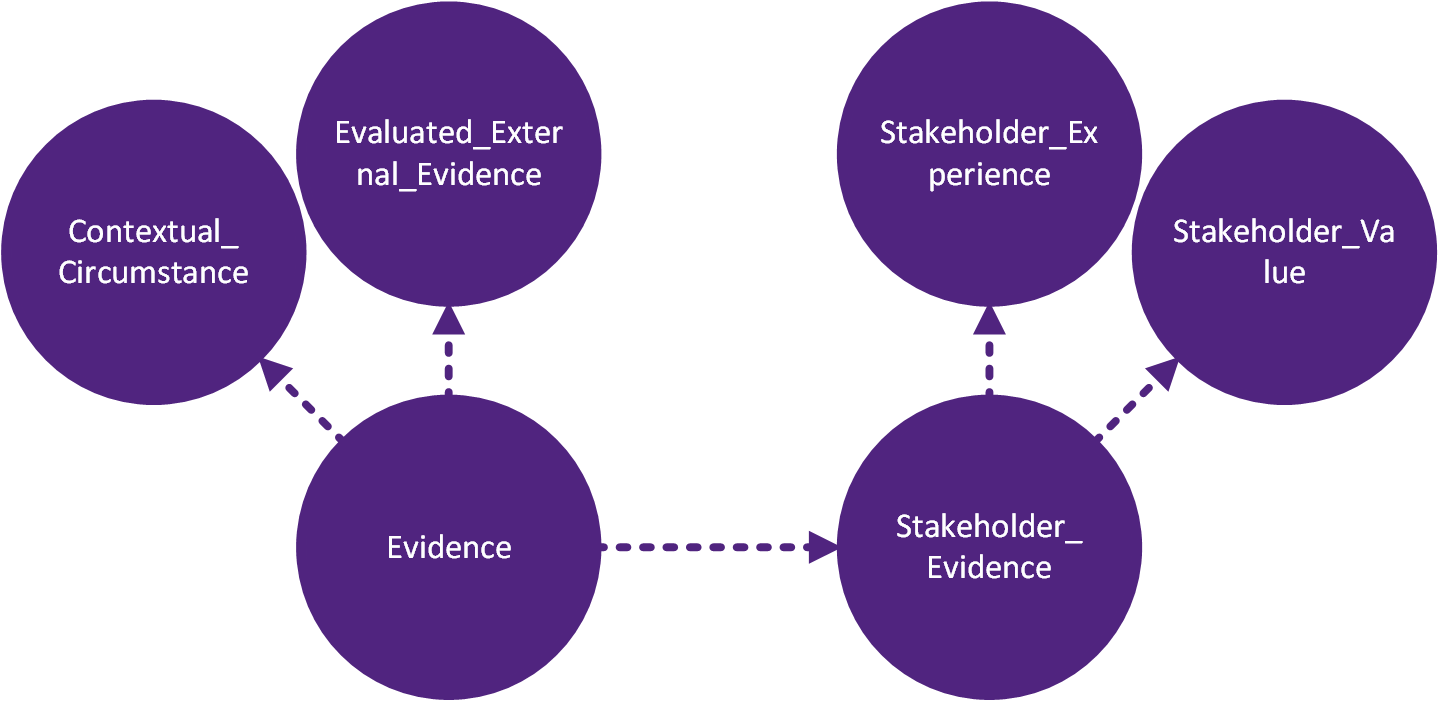
\includegraphics[width=9cm]{../../Images/04_Contribution/04_EBM_Classification.png}
  \caption{An overview of the evidence-based management ontology. $Stakeholder\_Experience$ and $Stakeholder\_Values$ as subclasses of $Stakeholder\_Evidence$. We add $Stakeholder\_Evidence$ as a subclass to $Evidence$ itself. Code sample \ref{GODP_EBM} presents the GDOL code that instantiates this ontology.}
  \label{fig:classification}
\end{figure} 

We create these classes for two purposes. First, the evidence spread determines the reproducibility of the evidence. The decision-maker can decide to gather additional evidence to increase the reproducibility of the decision-relevant information if, for example, the decision-relevant information is only based on $Stakeholder\_Experience$. Second, we extract $Contextual\_Circumstances$ from a written context or observation while we extract $Evaluated\_External\_Evidence$ from other written documents. We can reproduce this evidence based on its source. For $Stakeholder\_Evidence$, we need to know the stakeholder to reproduce it. Different evidence types have different behaviour and, therefore, need different classes.

\paragraph{Consistency}
We guard the consistency of the ontology using $DisjointClasses$. $Stakeholder\_Experience$ is logically different from $Stakeholder\_Value$. An individual cannot be $Stakeholder\_Evidence$, $Contextual\_Circumstance$, or $Evaluated\_External\_Evidence$ at the same time due to the difference in definition. When the reasoner classifies an individual as two disjoint classes, it will throw an inconsistency error and cannot continue reasoning. Figure \ref{fig:consistency_ebm} presents an example of an inconsistency error in Prot\'eg\'e. Code sample \ref{GODP_EBM} presents the implementation of the $DisjointClasses$.

\begin{figure}[H]
\centering
  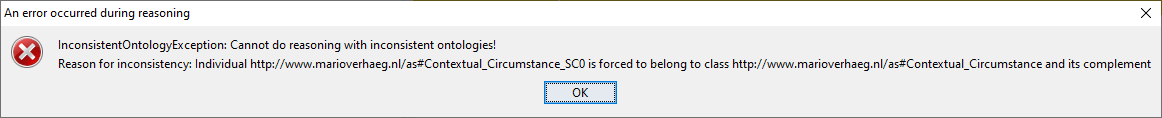
\includegraphics[width=17cm]{../../Images/04_Contribution/Consistency.png}
  \caption{An inconsistent ontology structure that a reasoner detects in Prot\'eg\'e. In this case, the individual $Contextual\_Circumstance\_SC0$ belongs to the classes $Contextual\_Circumstance$ and $Evaluated\_External\_Evidence$. $Contextual\_Circumstance\_SC0$ and $Evaluated\_External\_Evidence$ are disjoint classes. The reasoner does not accept that $Contextual\_Circumstance\_SC0$ belongs to both of these classes.}
  \label{fig:consistency_ebm}
\end{figure}

\paragraph{Inferencing}
The evidence-based management pattern uses a simple structure of classes and does not use inferencing to increase the amount of information in the ontology. 

\paragraph{Generic Ontology Design Pattern}
Code sample \ref{GODP_EBM} presents the generic ontology design pattern of the evidence-based management pattern using GDOL. We instantiate the evidence-based management pattern once per ontology it needs to extend. The evidence-based management pattern does not require parameters; therefore, we instantiate an $ontology$ instead of a $pattern$.

\begin{lstlisting}[float,language=GDOL,caption={The GDOL code that instantiates the generic ontology design pattern for evidence-based management. The instantiation includes the instantiation of the classes as well as the characteristics of those classes. Figure \ref{fig:classification} presents the structure of the pattern. },label={GODP_EBM}][H]
ontology EBM =
 Class: Evidence
 Class: Stakeholder
 Class: Stakeholder_Evidence SubClassOf: Evidence 
 Class: Stakeholder_Experience SubClassOf: Stakeholder_Evidence 
 Class: Stakeholder_Value SubClassOf: Stakeholder_Evidence 
 Class: Contextual_Circumstance SubClassOf: Evidence 
 Class: Evaluated_External_Evidence SubClassOf: Evidence 
 DisjointClasses: Stakeholder_Evidence, Contextual_Circumstance, Evaluated_External_Evidence	
 DisjointClasses: Stakeholder_Experience, Stakeholder_Value
\end{lstlisting}

\paragraph{Constraints}
It is possible to define constraints based on the stake of a specific evidence type. For example, the $Evaluated\_External\_Evidence$ should represent 20\% of the evidence related to a specific decision. However, these constraints would be very context-sensitive. We leave it up to the decision-maker to evaluate the mix of evidence-types manually on a case-by-case basis. Alternatively, the domain expert can manually add constraints based on the preference of the organisation implementing the decision design pattern.